\documentclass[slidetop,compress,mathserif]{beamer}
\usepackage[utf8]{inputenc}
\usepackage[french]{babel}
\usepackage{graphicx}
\usetheme{Antibes}
\usecolortheme{lily}
\title{Conception, implémentation et analyse d'un framework d'édition interactive d'images gigapixel.}
\author{Frédéric van der Essen \\ Promoteurs: Philip Dutré, Marc Lobelle.}

\begin{document}
	\begin{frame}
		\titlepage
	\end{frame}
	\section{Images Giga-Pixel}
	\begin{frame}
		\frametitle{Qu'est ce qu'une image Giga-Pixel ?}
		\begin{itemize}
			\pause \item Une image de plus d'un milliard de pixels indépendants
			\pause \item Une image trop grande pour tenir entièrement dans la mémoire vive.
		\end{itemize}
	\end{frame}
	\begin{frame}
		\frametitle{Applications des images Giga-Pixel}
		\begin{columns}
			\begin{column}{0.5\textwidth}
				\begin{itemize}
					\item<2-> La cartographie
					\item<3-> La numérisation d'oeuvres d'art
					\item<4-> La 3D photoréaliste
					\item<5-> Les jeux vidéos.
				\end{itemize}
			\end{column}
			\begin{column}{0.5\textwidth}
				\only<2>{
					\begin{figure}[h]
						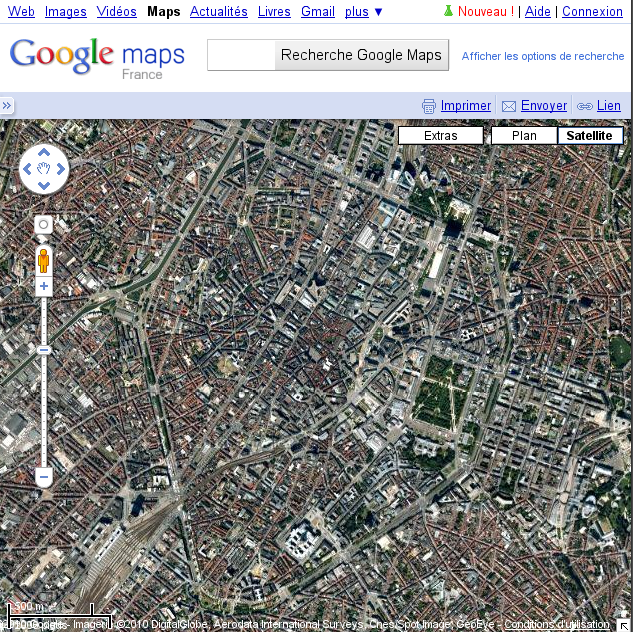
\includegraphics[width=\textwidth]{images/googlemaps}
					\end{figure}
				}
				\only<3>{
					\begin{figure}[h]
						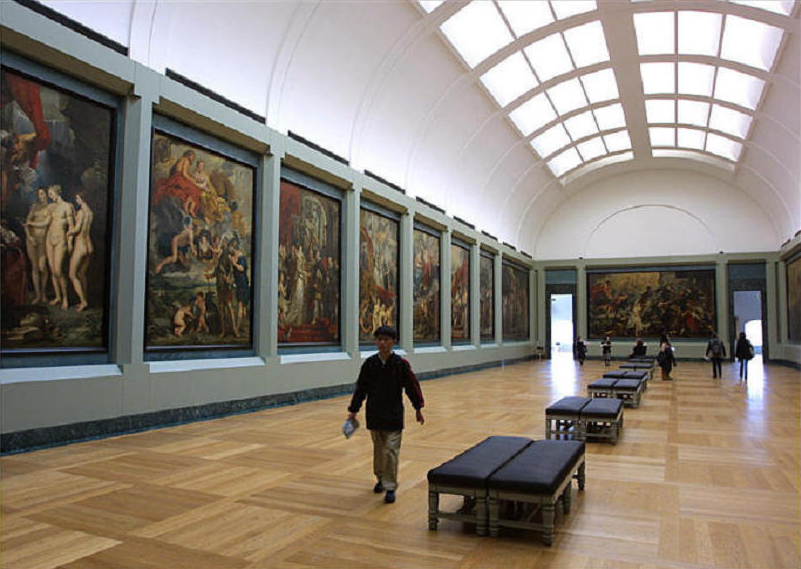
\includegraphics[width=\textwidth]{images/bigpaintings}
					\end{figure}
				}
				\only<4>{
					\begin{figure}[h]
						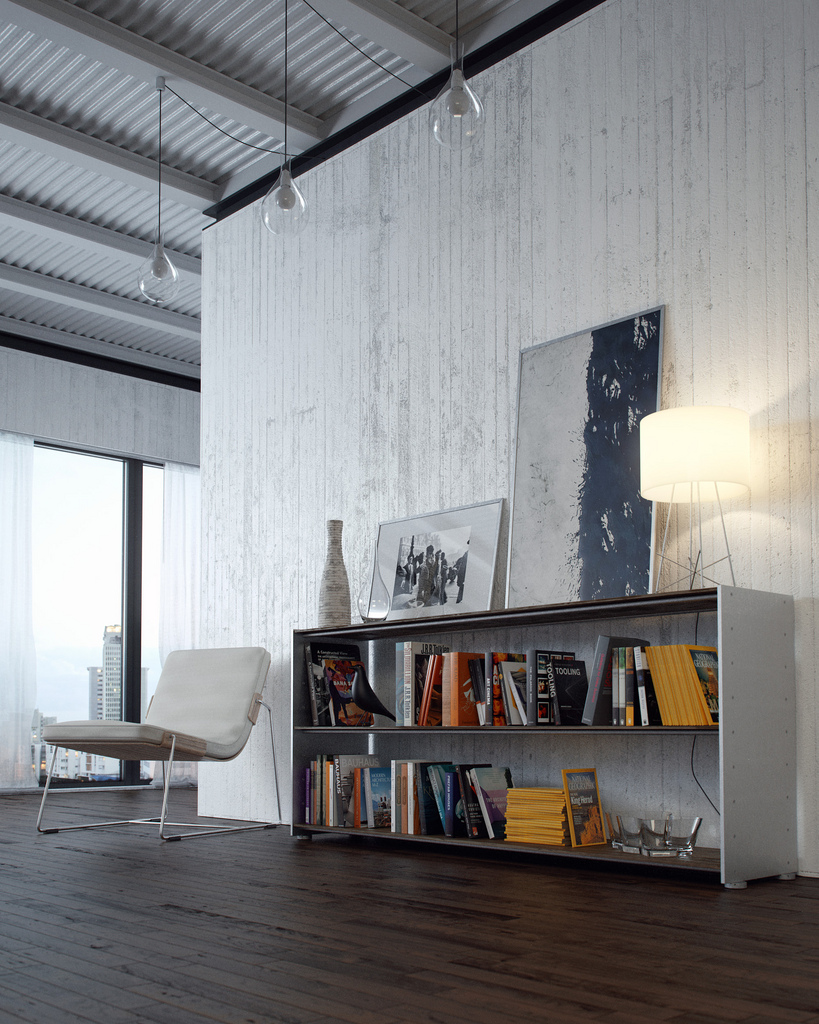
\includegraphics[width=\textwidth]{images/3darchitecturale}
					\end{figure}
				}
				\only<5>{
					\begin{figure}[h]
						\includegraphics[width=\textwidth]{images/rage}
					\end{figure}
				}
			\end{column}
		\end{columns}
	\end{frame}
	\begin{frame}
		\frametitle{Images Giga-Pixel: L'état de l'art}
		\pause
		\begin{itemize}
			\item On sait acquérir des images giga-pixel
			\pause
			\item On sait afficher des images giga-pixel
			\pause
			\item On sait stocker des images giga-pixel
			\pause
			\item Les possibilités d'éditions sont très limitées.
		\end{itemize}
	\end{frame}
	\section{Frameworks d'édition d'images}
	\begin{frame}{Composition d'un framework}
		\begin{itemize}
			\pause
			\item Une structure de représentation de l'image.
			\pause
			\item Des algorithmes d'édition de cette structure.
			\pause
			\item Un algorithme de rasterisation.
		\end{itemize}
	\end{frame}
	\begin{frame}
		\frametitle{Frameworks d'édition d'images}
		Il existe trois types de frameworks d'éditions d'images :
		\begin{itemize}
			\item Frameworks Bitmaps.
			\item Frameworks Vectoriels.
			\item Frameworks Nodaux.
		\end{itemize}
	\end{frame}
	\subsection{Frameworks Bitmaps}
	\begin{frame}{Frameworks Bitmaps}
		\begin{itemize}
		\item Représentation de l'image sous forme rasterisée.
		\item La rasterisation est faite à chaque modification de l'image.
			\pause
			\begin{itemize}
				\item $O(S)$, $S$ est le nombre de pixels affectés par l'opération.
			\end{itemize}
		\pause
		\item Les modifications ne sont pas retenues.
		\end{itemize}
	\end{frame}
	\begin{frame}{Avantages et Inconvénients}
		\begin{itemize}
			
			\item Avantages: 
			\begin{itemize}
				\item Grand nombre d'opérations.
				\item Édition pixel par pixel.
				\item Bonne interactivité à faible résolution.
			\end{itemize}
			\pause
			\item Inconvénients: 
			\begin{itemize}
				\item Résolution limitée: $\leq$ 100 Méga-Pixels
				\item Pas d'édition non destructive. 
			\end{itemize}
		\end{itemize}
	\end{frame}
	
	\begin{frame}{Usages}
		\begin{itemize}
			\item Peinture
			\item Retouche Photo
			\pause
			\item \emph{Adobe Photoshop}, \emph{The Gimp}, etc.
		\end{itemize}
	\end{frame}
	\subsection{Frameworks Vectoriels}
	\begin{frame}{Frameworks Vectoriels}
		\begin{itemize}
		\item Le dessin est composé de primitives
		\item Ces primitives sont représentées par un scene graph.
		\item La rasterisation est faite à chaque visualisation de l'image 
			\pause
			\begin{itemize}
				\item $O(s*n)$, $s$ la taille en pixel de la région à visualiser, $n$
				le nombre de primitives affectant la région.
			\end{itemize}
		\end{itemize}
	\end{frame}
	\begin{frame}{Avantages et Inconvénients}
		\begin{itemize}
			\item Avantages: 
			\begin{itemize}
				\item Indépendance à la résolution.
				\item Édition non destructive.
				\item Description compacte de l'image.
			\end{itemize}
			\pause
			\item Inconvénients: 
			\begin{itemize}
				\item Pas d'édition pixel par pixel
				\item Nombre limité de primitives. 
			\end{itemize}
		\end{itemize}
	\end{frame}
	
	\begin{frame}{Usages}
		\begin{itemize}
			\item Impression
			\item Documents structurés
			\item Interfaces graphiques
			\pause
			\item \emph{Adobe Illustrator}, \emph{Inkscape}, Navigateur Webs, Cette présentation ! 

		\end{itemize}
	\end{frame}
	\subsection{Frameworks Nodaux}
	\begin{frame}{Frameworks Nodaux}
		\begin{itemize}
		\item Représentation de l'image sous forme de graphe de modifications
		\item La rasterisation est faite à chaque visualisation de l'image. 
		\end{itemize}
	\end{frame}
	\begin{frame}{Avantages et Inconvénients}
		\begin{itemize}
			\item Avantages: 
			\begin{itemize}
				\item Édition non destructive.
				\item Édition non linéaire.
				\item Traitement de masse.
				\item Indépendance à la résolution.
				\item Combinaison avec d'autres frameworks.
			\end{itemize}
			\pause
			\item Inconvénients: 
			\begin{itemize}
				\item Nombre limité d'opérations.
				\item Algorithmes de modifications complexes à gérer.
			\end{itemize}
		\end{itemize}
	\end{frame}
	
	\begin{frame}{Usages}
		\begin{itemize}
			\item Post-Production Vidéo
			\item Retouche Photo
			\pause
			\item \emph{ Apple Shake}, \emph{Blender 3D}, \emph{The Gimp}
		\end{itemize}
	\end{frame}
	\subsection{Himalaya}
	\begin{frame}{Himalaya}
		Nouveau type de framework d'édition d'images.
		\begin{itemize}
			\pause
			\item Inspiration:
			\begin{itemize}
				\item Framework Nodaux.
				\item MegaTexturing
			\end{itemize}
			\pause
			\item Avantages: 
			\begin{itemize}
				\item Édition non destructive.
				\item Édition non linéaire.
				\item Édition pixel par pixel.
				\item Grand nombre d'opérations.
				\item Bonne interactivité à haute résolution.
			\end{itemize}
			\pause
			\item Inconvénients: 
			\begin{itemize}
				\item Filtres spatiaux.
			\end{itemize}
		\end{itemize}
	\end{frame}
	\section{Présentation du Framework Himalaya}
	\subsection{Frame}
	\begin{frame}{Tiles}
		\begin{columns}
			\begin{column}{0.5\textwidth}
				\begin{figure}[h]
					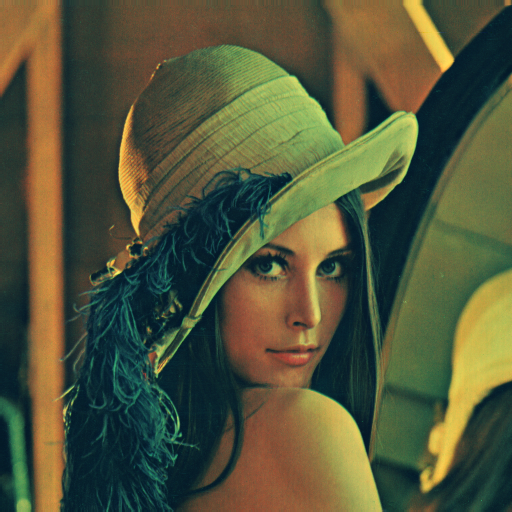
\includegraphics[width=\textwidth]{images/Lenna-green}
				\end{figure}
			\end{column}
			\begin{column}{0.5\textwidth}
				\pause
				\begin{figure}[h]
					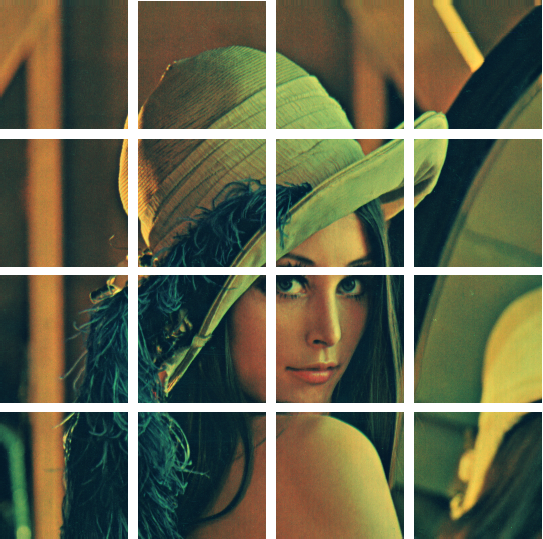
\includegraphics[width=\textwidth]{images/Lenna-green-grid}
				\end{figure}
			\end{column}
		\end{columns}
	\end{frame}
	\begin{frame}{MipMaps}
				\begin{figure}[h]
					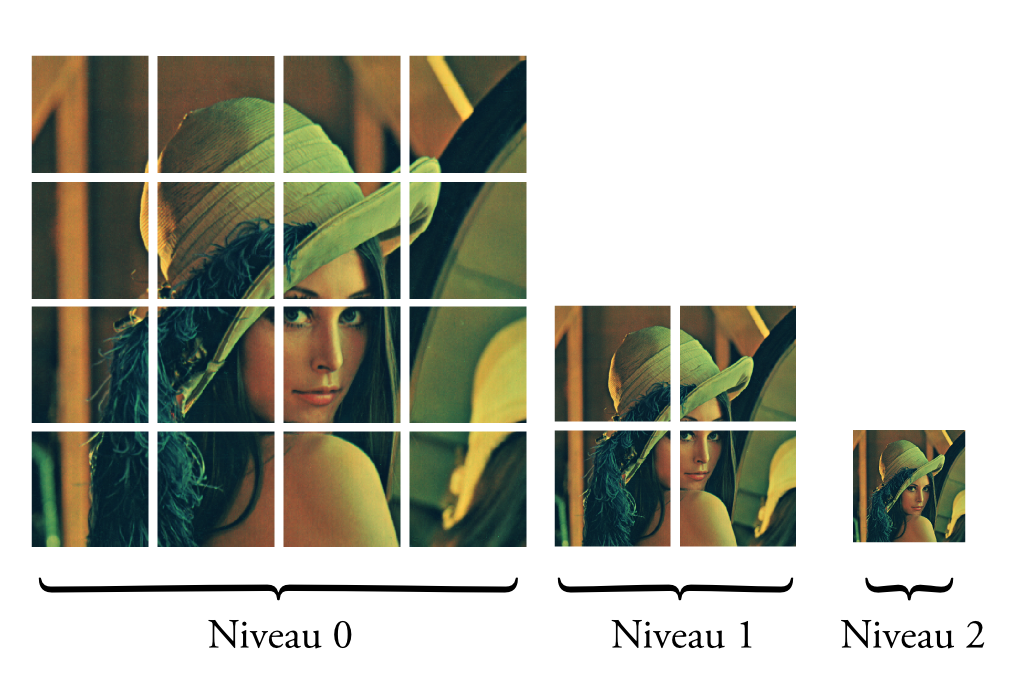
\includegraphics[width=0.6\textwidth]{images/tile-levels}
				\end{figure}
	\end{frame}
	\begin{frame}{Pyramide de tile creuse}
		\begin{columns}
			\begin{column}{0.5\textwidth}
				\begin{figure}[h]
					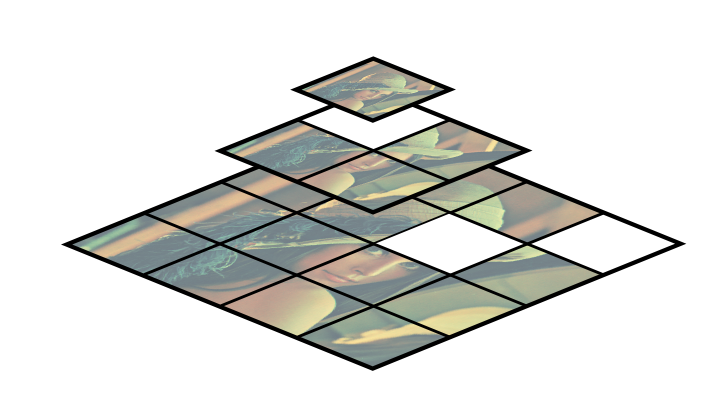
\includegraphics[width=\textwidth]{images/megatextures-pyramid-nouv}
				\end{figure}
			\end{column}
			\begin{column}{0.5\textwidth}
				\pause
				\begin{figure}[h]
					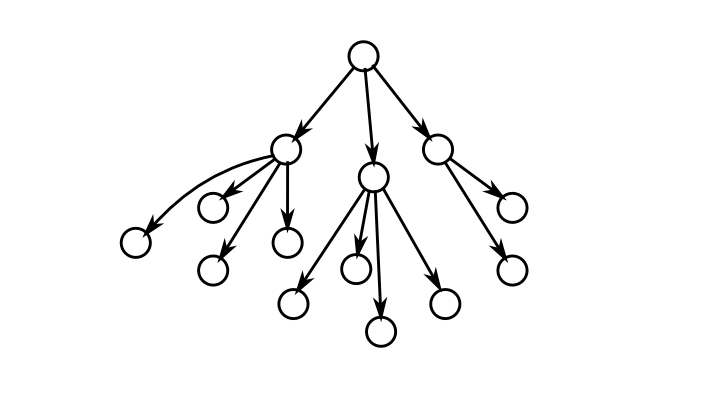
\includegraphics[width=\textwidth]{images/megatextures-pyramid-links}
				\end{figure}
			\end{column}
		\end{columns}
	\end{frame}
	\begin{frame}{hlFrame : Propriétés}
		\begin{itemize}
			\pause \item Accès, insertion et supression de tiles en $O(1)$
			\pause \item La profondeur de l'arbre reste optimale.
			\pause \item Pas de taille maximale. 
			\pause \item Les régions de couleur unie ne consomment pas de mémoire.
		\end{itemize}
	\end{frame}

	\begin{frame}{hlFrame : Utilité}
		\begin{itemize}
			\pause \item Stocker des bitmaps
			\pause \item Servir de cache aux opérations.
		\end{itemize}
	\end{frame}

	\subsection{Images}
	\begin{frame}{Images}
		Une image dans Himalaya c'est :
		\begin{columns}
			\begin{column}{0.3\textwidth}
				\begin{itemize}
					\item Un bitmap \emph{Source}
					\item Une pile d'opérations qui vont modifier ce bitmap.
				\end{itemize}
			\end{column}
			\begin{column}{0.7\textwidth}
				\pause
				\begin{figure}[h]
					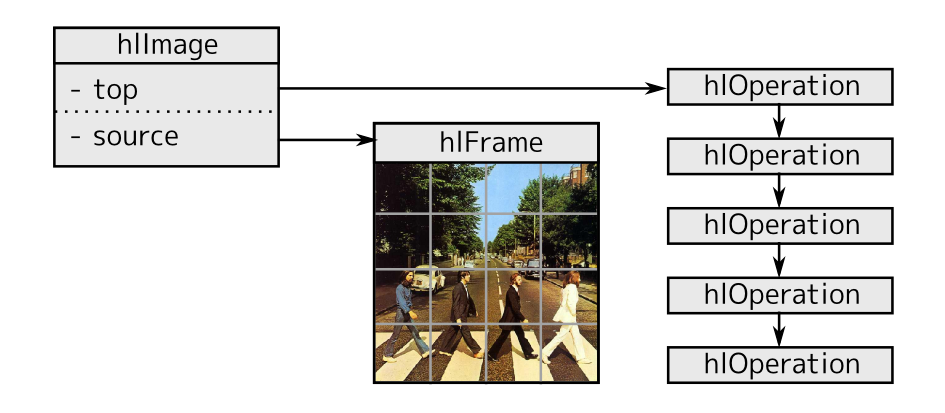
\includegraphics[width=\textwidth]{images/hlImage1}
				\end{figure}
			\end{column}
		\end{columns}
	\end{frame}	
	\begin{frame}{Rasterisation}
		\pause
		\begin{columns}
			\begin{column}{0.7\textwidth}
				\uncover<3->{ 
					hTile \emph{Rasterise}( operation, tile\_coord):
				}
				\begin{enumerate}
					\item<4-> Tile en Cache ? Renvoyer le tile
					\item<9-> Opération opaque ? Aller en \emph{4}
					\item<5-> hlTile T = \emph{Rasterise}(operation.down,tile\_coord)
					\item<6-> \emph{Draw}(operation,T)
					\item<7-> On met T en cache
					\item<8-> On renvoie T
				\end{enumerate}
			\end{column}
			\begin{column}{0.3\textwidth}
				\uncover<1->{
				\begin{figure}[h]
					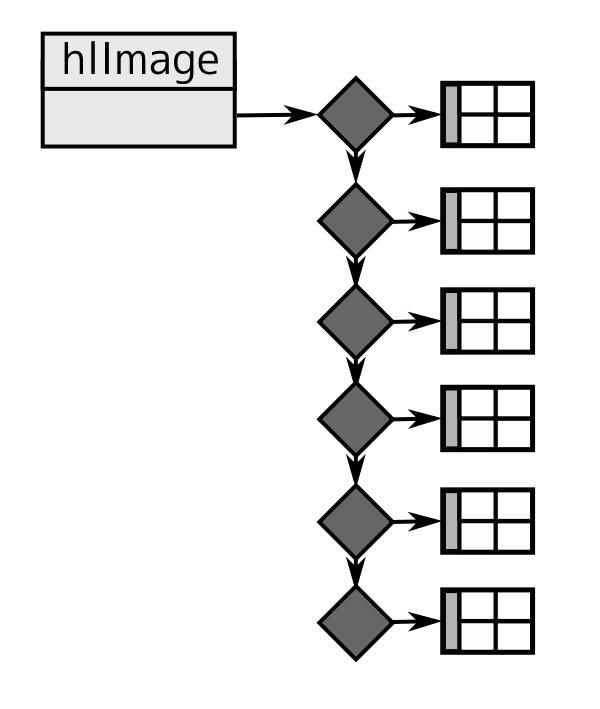
\includegraphics[width=\textwidth]{images/rasterisation}
				\end{figure}
				}
			\end{column}
		\end{columns}
	\end{frame}	
	\begin{frame}{Propriété de la Rasterisation}
		\begin{itemize}
		\item Complexité temporelle : $O(n)$ où $n$ est le nombre d'opérations
		non opaques
		ajoutées depuis la dernière rasterisation du tile.
		\item Rasteriser une région : $O(s*n)$ où $s$ est le nombre de tiles dans la région.
		\end{itemize}
	\end{frame}
	\begin{frame}{Ne pas mettre en cache à chaque opération}
		\begin{itemize}
			\item Ne cacher qu'à certaines opérations.
			\item Enlever de la cache avant le retour 
			lorsque l'opération ne doit plus cacher.
		\end{itemize}
	\end{frame}
	\begin{frame}{États}
		\begin{itemize}
			\item Permettre à l'utilisateur d'accéder à différentes 
			versions de son image.
		\end{itemize}
	\end{frame}
		
\end{document}
